% Exam Template for UMTYMP and Math Department courses
%
% Using Philip Hirschhorn's exam.cls: http://www-math.mit.edu/~psh/#ExamCls
%
% run pdflatex on a finished exam at least three times to do the grading table on front page.
%
%%%%%%%%%%%%%%%%%%%%%%%%%%%%%%%%%%%%%%%%%%%%%%%%%%%%%%%%%%%%%%%%%%%%%%%%%%%%%%%%%%%%%%%%%%%%%%

% These lines can probably stay unchanged, although you can remove the last
% two packages if you're not making pictures with tikz.
\documentclass[11pt]{exam}
\RequirePackage{amssymb, amsfonts, amsmath, latexsym, verbatim, xspace, setspace, graphicx, caption}


% By default LaTeX uses large margins.  This doesn't work well on exams; problems
% end up in the "middle" of the page, reducing the amount of space for students
% to work on them.
\usepackage[margin=1in]{geometry}
\usepackage[english]{babel}
\usepackage[autostyle]{csquotes} %%%% This package allows Tex to recognize quotation marks with the \enquote command. 


% Here's where you edit the Class, Exam, Date, etc.
\newcommand{\class}{MAT 132}
\newcommand{\term}{Summer II 2019}
\newcommand{\examnum}{Quiz 3}
\newcommand{\examdate}{07/31/19}
\newcommand{\timelimit}{50 minutes}

% For an exam, single spacing is most appropriate
\singlespacing
% \onehalfspacing
% \doublespacing

% For an exam, we generally want to turn off paragraph indentation
\parindent 0ex
\title{MAT 132 - Summer II 2019: Quiz 3 solutions}
\begin{document} 

% These commands set up the running header on the top of the exam pages
\pagestyle{head}
\firstpageheader{}{}{}\textbf{}
\runningheader{\class}{\examnum\ - Page \thepage\ of \numpages}{\examdate}
\runningheadrule

\begin{flushright}
\begin{tabular}{p{2.8in} r l}
\textbf{\class} & \textbf{Name (Print):} & \makebox[2in]{\hrulefill}\\
\textbf{\term} &&\\
\textbf{\examnum} &&\\
\textbf{\examdate} &&\\
\textbf{Time Limit: \timelimit} & ID number & \makebox[2in]{\hrulefill}
\end{tabular}\\
\end{flushright}
\rule[1ex]{\textwidth}{.1pt}

\begin{center}
\large{\textbf{Instructions}}
\end{center}

\begin{minipage}[t]{3.7in}
\vspace{0pt}
\begin{itemize}

\item This exam contains \numpages\ pages (including this cover page) and
\numquestions\ problems.  Check to see if any pages are missing.  Enter
all requested information on the top of this page, and put your initials
on the top of every page, in case the pages become separated.

\item You may \textit{not} use your books, notes, or any device that is capable of accessing the internet on this exam (e.g., smartphones, smartwatches, tablets). You may use a calculator.

\item \textbf{Organize your work}, in a reasonably neat and coherent way, in
the space provided. Work scattered all over the page without a clear ordering will 
receive very little credit.  

\item \textbf{Mysterious or unsupported answers will not receive full
credit}.

\end{itemize}

\end{minipage}
\hfill
\begin{minipage}[t]{2.3in}
\vspace{0pt}
%\cellwidth{3em}
\gradetablestretch{2}
\vqword{Problem}
\addpoints % required here by exam.cls, even though questions haven't started yet.	
\gradetable[v]%[pages]  % Use [pages] to have grading table by page instead of question

\end{minipage}
\newpage % End of cover page

%%%%%%%%%%%%%%%%%%%%%%%%%%%%%%%%%%%%%%%%%%%%%%%%%%%%%%%%%%%%%%%%%%%%%%%%%%%%%%%%%%%%%
%
% See http://www-math.mit.edu/~psh/#ExamCls for full documentation, but the questions
% below give an idea of how to write questions [with parts] and have the points
% tracked automatically on the cover page.
%
%
%%%%%%%%%%%%%%%%%%%%%%%%%%%%%%%%%%%%%%%%%%%%%%%%%%%%%%%%%%%%%%%%%%%%%%%%%%%%%%%%%%%%%

\begin{questions}

% Basic question
%%%%%%%%%%%%%%

%%%%%%%%%%%%%%%%% 

\addpoints
\question Match the differential equations and slope fields below. Explain your reasoning in the space provided below each equation.   

\begin{figure}[h]
\centering
\begin{minipage}{.5\textwidth}
  \centering
  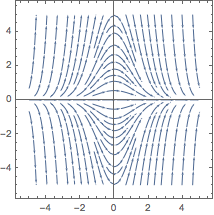
\includegraphics[width=.4\linewidth]{slopefield3}
  \caption{Slope field 1}
  %\label{fig:test3}
\end{minipage}%
\begin{minipage}{.5\textwidth}
  \centering
  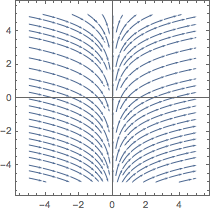
\includegraphics[width=.4\linewidth]{slopefield2}
  \caption{Slope field 2}
 %\label{fig:test2}
\end{minipage}
\end{figure}

\begin{parts}
\part[1]
\begin{equation*}
y'=-xy
\end{equation*} 

\textbf{Solution:} Solutions to this equation have slope $y'=0$ whenever $x=0$ or $y=0$. The figure that matches this behavior is Figure 1. 
\vfill
\part[1] 

\begin{equation*}
y'=\frac{1}{x} 
\end{equation*}
\textbf{Solution:} Solutions to this equation have discontinuous slopes, as 
\begin{equation*}
|y'| \to \infty
\end{equation*}
when $x \to 0$. The figure that matches this behavior is Figure 2. 
\vfill
\end{parts}
%%%%%%%%%%%%%%%%%

\newpage
\addpoints
\question[4] Consider the initial-value problem
\begin{align*}
y'(x) & = x+y, \\
y(0) & = 1.
\end{align*}
Estimate the value of $y(1)$ using Euler's method with $4$ steps.  

\textbf{Solution:} The step size for Euler's method is 
\begin{equation*}
\Delta x = 0.25.
\end{equation*}
We'll use Euler's formula for the succesive approximations, and round off results to three decimal places when necessary.

The first approximation is 
\begin{equation*}
y_1=y_0+0.25 \cdot y^{'}_{0} = 1+0.25\cdot 1 = 1.25.
\end{equation*}

The slope at the point $(x_1,y_1)=(0.25, 1.25)$ is $y^{'}_{1}=1.5$. We use this to find the second approximation, 
\begin{equation*}
y_2=y_1+0.25 \cdot y^{'}_{1} = 1.25+0.25\cdot 1.5 = 1.625.
\end{equation*}

The slope at the point $(x_2,y_2)=(0.5, 1.625)$ is $y^{'}_{2}=2.125$. We use this to find the third approximation, 
\begin{equation*}
y_3=y_2+0.25 \cdot y^{'}_{2} = 1.625+0.25\cdot 2.125 \approx 2.156.
\end{equation*}

The slope at the point $(x_3,y_3)=(0.75, 2.156)$ is $y^{'}_{3}=2.906$. We use this to find the fourth and final approximation, 
\begin{equation*}
y_4=y_3+0.25 \cdot y^{'}_{3} = 2.156 +0.25\cdot 2.906 \approx 2.883.
\end{equation*}
%%%%%%%%%
\newpage
\addpoints

\question A population $P(t)$ satisfies the initial-value problem
\begin{equation*}
\frac{dP}{dt} = 0.4P - 0.001P^2, \ \ P(0)=50.
\end{equation*}
\begin{parts}
\part[3] Find $P(t)$. 

\textbf{Solution:} We start by rewritting the equation as
\begin{equation*}
\frac{dP}{dt} = \frac{P(400-P)}{1000}.
\end{equation*}
Now we can separate variables and integrate, 
\begin{equation}
\label{equation_integrated}
\int \frac{1000}{P(400-P)} \ dP = \int 1 \ dt. 
\end{equation}
The integral on the left-hand side requires integration by partial fractions. The partial fractions decomposition is 
\begin{equation*}
\frac{1000}{P(400-P)} = \frac{2.5}{P} + \frac{2.5}{400-P}.
\end{equation*}
Now we can find an antiderivative for the integral, 
\begin{align*}
\int \frac{1000}{P(400-P)} \ dP & = \int \frac{2.5}{P} \ dP + \int \frac{2.5}{40-P} \ dP\\
& = 2.5\ln(|P|) - 2.5\ln(|400-P|).
\end{align*}
Substituting into equation \eqref{equation_integrated}, we obtain
\begin{equation}
\label{equation_missing_C}
2.5[\ln(|P|) - 2.5\ln(|400-P|) = t+C .
\end{equation}
At this point, we are in a position to find the constant $C$. We can do so by substituting $P(0)=50$, 
\begin{equation*}
C = 2.5\ln\left(\frac{50}{350}\right)=-2.5\ln(7).
\end{equation*}
Substituting this into \eqref{equation_missing_C}, we obtain 
\begin{equation*}
2.5[(\ln(|P|)-\ln(|400-P|)] = t- 2.5\ln(7), 
\end{equation*}
and by exponentiation, 
\begin{equation*}
\left| \frac{P}{400-P}\right| = \frac{e^{\frac{t}{2.5}}}{7}.
\end{equation*}
Here we note that the initial condition $P(0)=50$ lies below the equilibrium solution $P_{eq}(t)=400$, hence $P(t) <400$, for all $t >0$. It follows that 
\begin{equation*}
\frac{P}{400-P}=\frac{e^{\frac{t}{2.5}}}{7}.
\end{equation*}
\newpage 

Solving this equation for $P$ yields 
\begin{equation*}
P(t)=\frac{400e^{\frac{t}{2.5}}}{7+e^{\frac{t}{2.5}}}.
\end{equation*}

\part[1] What is the limiting value for the population when $t \to \infty$?

\textbf{Solution:}
This can be done by taking the limit of the expression found in part(a), 
\begin{align*}
\lim_{t \to \infty} P(t) & = \lim_{t \to \infty} \frac{400e^{\frac{t}{2.5}}}{7+e^{\frac{t}{2.5}}} \\ 
& = 400.
\end{align*}
\end{parts}
\addpoints 

%%%%%%%%%%%%
\newpage
\question[4]  Solve the following first-order equation
\begin{equation*}
y'(x)+xy(x)=x.
\end{equation*}

\textbf{Solution:} An integrating factor of the equation is given by 
\begin{equation*}
\mu(x)=e^{\int x dx} = e^{\frac{x^2}{2}}.
\end{equation*}
Multiplying the equation by this factor, we obtain
\begin{equation*}
(e^{\frac{x^2}{2}}y(x))'= xe^{\frac{x^2}{2}}.
\end{equation*}
Integrating both sides we get 
\begin{align*}
e^{\frac{x^2}{2}}y(x) & = \int xe^{\frac{x^2}{2}} \\
& = \int e^{u} du, \ \ \mbox{where} \ u = \frac{x^2}{2}, \\
& = e^{u}+C \\
& = e^{\frac{x^2}{2}}+C.
\end{align*}
It follows that the equation is solved by 
\begin{equation*}
y(x)=1+Ce^{-\frac{x^2}{2}}.
\end{equation*}
\addpoints

%%%%%%%%%%%%%%%
\newpage
\question Solve the following second-order equations
\begin{parts}
\part[2] $y''-5y'+6y=0$.

\textbf{Solution:} The characteristic equation of the problem is 
\begin{equation*}
r^2-5r+6=0,
\end{equation*}
and its solutions are $r=2$, $r=3$. Thus, the solutions of the differential equation are 
\begin{equation*}
y(x)=Ae^{2x}+Be^{3x}.
\end{equation*}
\vfill
\part[2] $y''+4y'+4y=0$. 

\textbf{Solution:} The characteristic equation of the problem is 
\begin{equation*}
r^2+4r+4=0.
\end{equation*}
This solution has a unique solution, with multiplicity 2, $r=-2$. It follows that the solutions of the differential equation are 
\begin{equation*}
y(x)=Ae^{-2x}+Bxe^{-2x}.
\end{equation*}
\vfill 
\newpage 
\part[2] $y'' + 4y=0$. 

\textbf{Solution:} The characteristic equation
\begin{equation*}
r^2+4=0
\end{equation*} 
does not have real solutions. In this case, the solutions are the complex numbers $2i$ and $-2i$. The corresponding solutions of the differential equation, written in complex form, are 
\begin{equation*}
y(x)=Ae^{2ix}+Be^{-2ix}.
\end{equation*}
In real form, the solutions become 
\begin{equation*}
y(x)=C\cos(2x)+D\sin(2x).
\end{equation*}
\addpoints
\end{parts}

\end{questions}
\end{document}
